\documentclass[10pt,twocolumn,letterpaper]{article}
\usepackage{cvpr}
\usepackage{times}
\usepackage{latin1}
\usepackage{epsfig}
\usepackage{graphicx}
\usepackage{amsmath}
\usepackage{amssymb}
\usepackage[utf8]{inputenc} 
\usepackage[breaklinks=true,bookmarks=false]{hyperref}
\usepackage{epstopdf}
\cvprfinalcopy % *** Uncomment this line for the final submission
\def\cvprPaperID{****} % *** Enter the CVPR Paper ID here
\def\httilde{\mbox{\tt\raisebox{-.5ex}{\symbol{126}}}}

% Pages are numbered in submission mode, and unnumbered in camera-ready
%\ifcvprfinal\pagestyle{empty}\fi
\setcounter{page}{1}
\begin{document}

%%%%%%%%% TITLE
\title{VLFeat como librería “open source”, modificación y evaluación de la función phowcaltech101 para la clasificación del conjunto de datos imagenet-tiny variando diferentes parámetros.}

\author{David L. Henao\\
\begin{normalsize}
Grupo de Ingeniería Biomédica. Universidad de los Andes, Bogotá, Colombia
\end{normalsize}
\\
{\tt\small dl.henao909@uniandes.edu.co}}
% For a paper whose authors are all at the same institution,
% omit the following lines up until the closing ``}''.
% Additional authors and addresses can be added with ``\and'',
% just like the second author.
% To save space, use either the email address or home page, not both
\maketitle
%\thispagestyle{empty}

%%%%%%%%% ABSTRACT
\begin{abstract}

En la práctica del laboratorio PHOW se aplicó y se evaluó la función phow\_caltech101 () (escrita por Andrea Vedaldi). Esta función emplea la librería VLFeat, la cual es una librería “open source” que implementa algorítmos populares, especializados en comprensión de imágenes y características locales de extracción y combinación.
La función phow\_caltech101() usa un SIFT denso (con el que se obtiene un descriptor SIFT en cada punto), histogramas espaciales y un support vector machine con la distancia chi 2. Cuando se ejecuta la función con la base de datos caltech101, esta entrena un clasificador y lo prueba con un subconjunto de imágenes de la misma. Si la base de datos no se encuentra disponible, el script automáticamente descarga una copia de la web.
En la práctica de laboratorio, se realizaron una serie de modificaciones a la función phow\_caltech101 para poder emplearla en una nueva base de datos “imagenet\_tiny”. Seguidamente, se realizó una evaluación del desempeño de la función tanto para caltech101 como para imagenet\_tiny. Dicha evaluación se realizó teniendo en cuenta la diagonal de la matriz de confusión variando 3 diferentes parámetros: Número de imágenes de entrenamiento, número de categorías y cambios en la partición espacial.
   
\end{abstract}

%%%%%%%%% BODY TEXT
\section{Introducción}

La investigación actual en visión computacional se construye a partir de algoritmos de visión y aprendizaje de máquinas estblecidos. Por ejemplo: la extracción de características, el agrupamiento y el aprendizaje. La mayoría de estos algoritmos base son relativamente nuevos y experimentales y cuando su implementación está disponible, usualmente sólo se encuentra en la forma binaria y para algunas plataformas específicas. Esta falta de disponibilidad de código fuente genera restricciones que impiden la adopción de nuevos algoritmos, pero más importante aún hace dificil aprender los detalles del algoritmo y modificarlos para poner en práctica nuevas ideas de investigación.[1]

Con esta motivación, Vedaldi y Fulkerson crearon la librería VLFeat. Esta, es una librería “open source” portable que incluye algoritmos de visión computacional. Su objetivo es facilitar la creación de prototipos rápidos y reproducibles por estudiantes y científicos de la visión por computador. Esta librería incluye implementaciones rigurosas de bloques de construcción como: detectores de características, extractores de características, agrupamiento por kmeans (jerárquico), árboles kd aleatórios y super-pixelación. Adicionalmente, esta librería se integra directamente con el software matlab que es ampliamente usado en esta área de investigación [1].

Por su parte, la función phow\_caltech101() realiza una categorización de imágenes: primero usa un detector SIFT (transformada de características invariante a escala )denso obteniendo así algunos descriptores PHOW para entrenar el vocabulario, luego computa los histogramas espaciales de forma paralela para realizar una posterior comparación de la distancia chi2 y  entrena el clasificador mediante SVM con la base de datos caltech101. Toda vez que se ejecuta la función con la base de datos, esta prueba el clasificador empleando un subconjunto de imágenes de la misma, calcula la matriz de confusión y muestra la precisión del clasificador partiendo de esta [2].

En este documento, se reportan los resultados obtenidos durante la práctica de laboratorio. Se realizaron una serie de modificaciones a la función phow\_caltech101 para poder emplearla en una nueva base de datos “imagenet\_tiny” y se realizó una evaluación del desempeño de la función tanto para caltech101 como para imagenet\_tiny teniendo en cuenta la precisión del clasificador otorgada por la diagonal de la matriz de confusión. Durante la práctica, se realizó la variación de 3 diferentes parámetros: Número de imágenes de entrenamiento, número de categorías y cambios en la partición espacial. Esto para determinar como modificaban dichos factores el rendimiento del clasificador en cuanto a precisión, tiempo y recursos computacionales [3].

%------------------------------------------------------------------------
\section{Metodología}

A continuación se presenta la metodología que lleva a cabo el algoritmo y las modificaciones implementadas en el método.

\subsection{¿Cómo funciona phow\_caltech101 () ?}

phow\_caltech101 consta de 5 diferentes secciones:\\

1. Extracción de características: Se emplea la función vl\_dsift para computar eficientemente un grupo denso de descriptores multiescala SIFT desde una imagen de entrada dada (descriptores PHOW[4]). Aunque la función vl\_sift de la librería también puede ser empleada para este propósito, con vl\_dsift se obtiene un descriptor en cada localización y se colectan más características incrementando a su vez la precisión en el reconocimiento. Adicionalmente, la función vl\_dsift es un orden de magnitud más rápida que vl\_sift [1].\\

2. Aprendizaje de vocabulario: Se emplea la función vl\_kmeans para agrupar cientos de miles de descriptores visuales en un vocabulario de 10\^3 palabras visuales. En esta función, se implementa el algoritmo de Elkan que para esta tarea es mucho más rápido que el algoritmo de Lloyd y varios órdenes de magnitud más rápido que la función kmeans nativa de matlab [1]. En la figura 1 se muestra un arbol jerárquico de kmeans hallado a partir de un conjunto de datos uniformemente distribuidos en un cuadrado. Kmeans puede ser empleado para construir grandes y eficientes vocabularios de palabras visuales [1].\\

\begin{figure}[t]
\begin{center}
%\fbox{\rule{0pt}{2in} \rule{0.9\linewidth}{0pt}}
   \includegraphics[width=0.9\linewidth]{f1_kmeans.png}
\end{center}
   \caption{Arbol jerárquico Kmeans datos uniformemente distribuidos en un cuadrado . Extraida de [1].}
\label{fig:seg}
\end{figure}

3. Histogramas espaciales: En la siguiente sección, se construye un histograma espacial, el cual caracteriza la distribución conjunta de la apariencia y la localización de las palabras visuales de la imagen [5]. Para ello se emplea la función vl\_kdtreequery que se emplea para asignar los descriptores a las palabras visuales de una manera eficiente empleando el un arbol KD.\\

4. Entrenar un SVM no lineal: Los histogramas espaciales son usados como descriptores de imágenes y alimentan a un clasificador lineal SVM, estos son muy rápidos de entrenar [6]. Sin embargo, se pueden tener mejores resultados transformando previamente los datos a través de vl\_homkermap. Esta función calcula una característica explícita que emula un kernel no lineal en uno lineal [7]. Luego se entrenan 15 imágenes para cada una de las 101 categorías de Caltech101 empleando vl\_pegasos, una implementación de un entrenamiento SVM de gradiente estocástico.\\

5. Evaluación del SVM cuyos resultados se discuten más adelante en la sección de discusión.


\subsection{¿Qué modificaciones se realizaron a phow\_caltech101 () ?}

Para poder emplear phow\_caltech101 y evaluar su desempeño en el conjunto de datos de imagenet\_tiny se realizaron las siguientes 4 modificacioens al algortimo:\\

1. Se le dió un valor de falso a la variable inicial que permitía descargar automáticamente la base de datos caltech101 de la web. Igualmente se comentarió la sección para evitar que el programa lanzara un error y se continuara ejecutando.\\

2. Se copió la carpeta de imagenet\_tiny que contenía el conjunto de imágenes en el directorio data y cambió el valor de la variable  dataDir por data/imagenet\_tiny/train.\\

3. Como las imágenes de imagenet\_tiny se encuentran en formato .JPEG y no en .jpg como es el caso de las imágenes de caltech101, también fue necesario modificar esta línea de código en la sección de preparamiento de datos.\\

4. Finalmente se añadieron diferentes cronómetros en las secciones de entrenamiento de vocabulario y del SVM así como en la sección de test del SVM. Esto, para evaluar en donde se esta llevando a cabo el mayor gasto de tiempo en el algoritmo.\\

En la figura 2 se puede observar la clasificación y el desempeño realizado por phow\_caltech101

\begin{figure}[t]
\begin{center}
%\fbox{\rule{0pt}{2in} \rule{0.9\linewidth}{0pt}}
   \includegraphics[width=1\linewidth]{f2_confusion.png}
\end{center}
   \caption{Ejemplo de categorización de Caltech-101. (a) Algunas imágenes del conjunto de datos de Caltech101 y (b) la matriz de confusión obtenida realizando el procedimiento descrito en la metodología.}
\label{fig:seg}
\end{figure}

%------------------------------------------------------------------------
\section{Resultados}

En las figuras 3 y 4 se pueden observar las curvas obtenidas para las diferentes precisiones.

Las curvas de la figura 3 fueron obtenidas, realizando en total 32 entrenamientos y clasificaciones, 16 para cada conjunto de datos (Caltech101 y Imagenet-tiny). Caltech101 obtiene resultados de precisión de hasta el 70.72\%, mientras que para Imagenet el máximo resultado obtenido es de 32.59\%. Es importante resaltar que en estos entrenamientos, el número de clases para ambos conjuntos de datos fue de 102 (el máximo que se puede colocar en caltech101) lo cual puede influir en el desempeño de Imagenet-tiny que tiene un número de máximo 200 clases.

\begin{figure}[t]
\begin{center}
%\fbox{\rule{0pt}{2in} \rule{0.9\linewidth}{0pt}}
   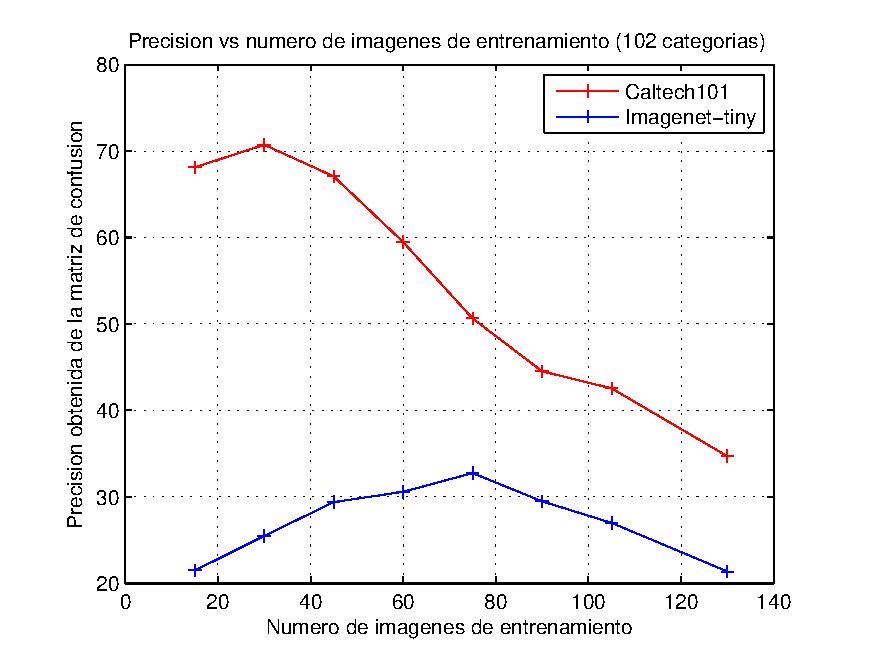
\includegraphics[width=1\linewidth]{train.eps}
\end{center}
   \caption{Precisión vs numero de imagenes de entrenamiento manteniendo 102 categorias para ambos conjuntos de datos.}
\label{fig:seg}
\end{figure}

Por otra parte, las curvas de la figura 4 fueron obtenidas, realizando en total 20 entrenamientos y clasificaciones, 16 para el conjunto de datos de Imagenet-tiny y 4 para Caltech101. Para este caso, Caltech101 obtiene resultados de precisión de hasta el 70.72\%, mientras que para Imagenet el máximo resultado obtenido es de 32.59\%. Es importante resaltar que en estos entrenamientos, el número de clases para ambos conjuntos de datos fue de 102 (el máximo que se puede colocar en caltech101) lo cual puede influir en el desempeño de Imagenet-tiny que tiene un número de máximo 200 clases.

\begin{figure}[t]
\begin{center}
%\fbox{\rule{0pt}{2in} \rule{0.9\linewidth}{0pt}}
   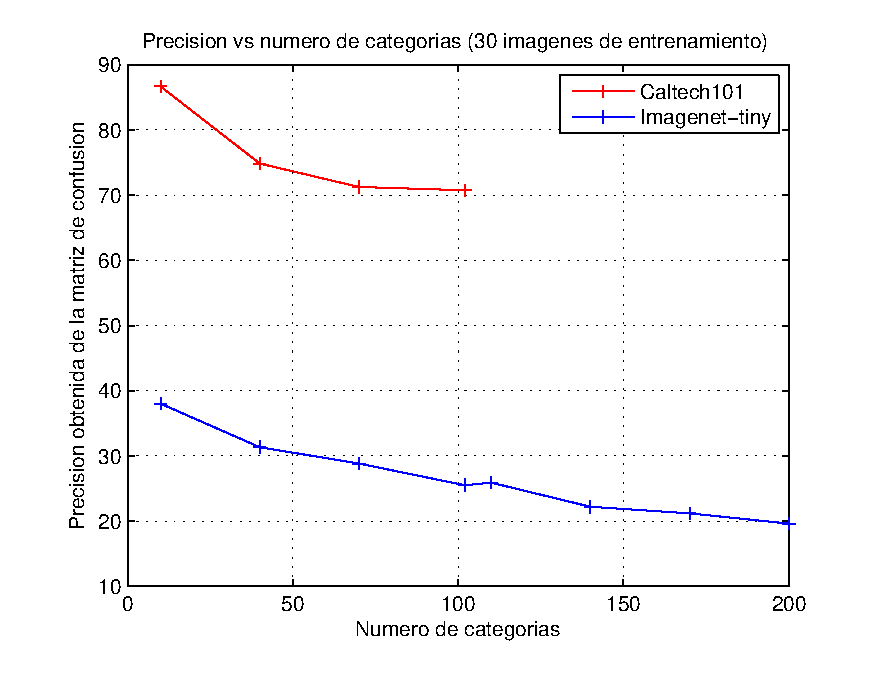
\includegraphics[width=1\linewidth]{cat.eps}
\end{center}
   \caption{Precisión vs numero de categorías manteniendo 30 imágenes de entrenamiento para ambos conjuntos de datos.}
\label{fig:seg}
\end{figure}

Ahora bién respecto a los resultados de tiempo, se muestra en la figura 5 una gráfica construida con los diferentes tiempos ( entrenamiento del vocabulario, construcción del histograma, entrenamiento del Support Vector Machine y prueba de Support Vector Machine) . Está gráfica se generó variando el número de imágenes de entrenamiento y tomando para cada entrenamiento (16 en total) el tiempo de cada una de esta etapas. Se empleó para dicha prueba el conjunto de datos de Caltech101 con un número de categorías de 102.

\begin{figure}[t]
\begin{center}
%\fbox{\rule{0pt}{2in} \rule{0.9\linewidth}{0pt}}
   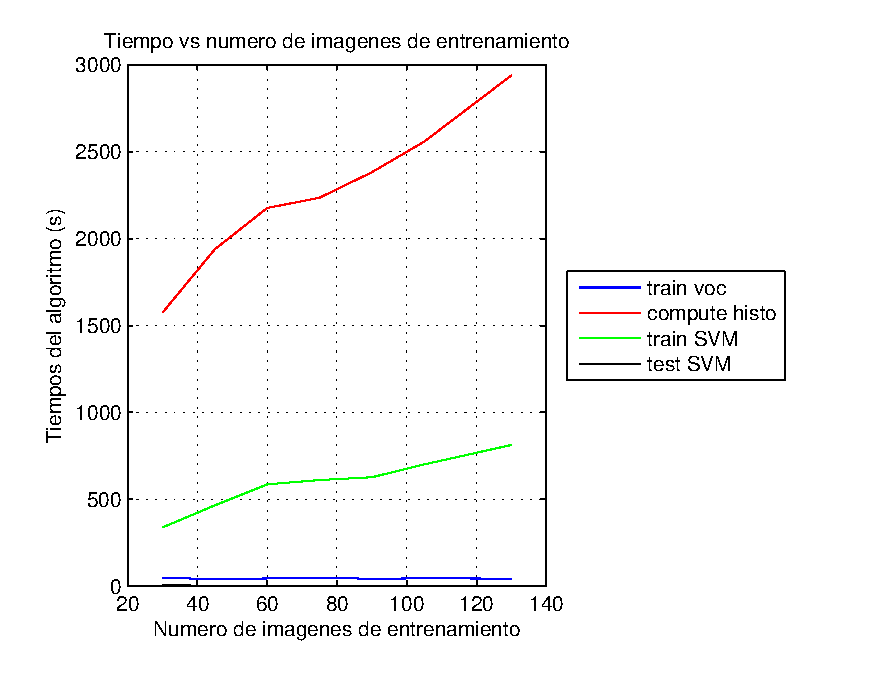
\includegraphics[width=1\linewidth]{time.eps}
\end{center}
   \caption{Tiempo empleado para cada una de las etapas del algoritmo variando el número de imágenes de entrenamiento. Base de datos Caltech101 con 102 categorías.}
\label{fig:seg}
\end{figure}

%------------------------------------------------------------------------
\section{Discusión}

En el momento de adaptar el algoritmo para trabajar en el nuevo conjunto de datos, se obtuvo un rendimiento (tomándo este como la precisión de clasificación) de 21.50\%. Este fue 46,6\% inferior al rendimiento de base obtenido con Caltech101, se puede explicar este primer fenómeno debido al número de categorías, ya que Imagenet\_tiny tiene un número total de 200 categorías mientras que Caltech101 tiene 102 categorías. Al entrenar el nuevo conjunto de datos con un número de categorías que no está acorde a este, puede reducir la presición de su clasificación. Por otro lado, el número de imágenes de entrenamiento para cada categoría se mantuvo en 15, esto también puede afectar el rendimiento, en el sentido de que pow\_caltech101 está configurado para correr un número de imágenes pequeño por lo que tiene un rendimiento del 68,10\% a pesar del número de imágenes de entrenamiento reducido. Sin embargo, no es el caso de Imagenet.

Con Caltech101 al aumentar el número de categorías inicialmente se aumenta la precisión de los resultados pero en general la precisión obtenida de la matriz de confunsión disminuye. Igualmente, con Imagenet-tiny la precisión se hace menor al aumentar el número de categorías, obteniendose la menor precisión (20) con 200 categorías. Además, se observó que con Caltech101 se obtiene una precisión significativamente mayor que con Imagenet-tiny, para los 4 números de categorías evaluados, con diferencias entre 49\% y 42\% aproximadamente. Se encontró que la razón de decaimiento de precisión con respecto al número de categorías es mayor con Caltech101 y que además tiene un comportamiento el cual podría ser descrito con una función polinómica. Asimismo, el comportamiento de la precisión obtenida con Imagenet-tiny en relación con  el aumento del número de catergorías se puede describir como una función lineal. 


Al aumentar el número de imágenes de entrenamiento en los 4 casos (train voc, compute histo, train SVM y test SVM) el tiempo aumenta, siendo significativamente mayor con train voc y train SVM. El menor tiempo fue encontrado con test SVM y el mayor tiempo con compute histo. La diferencias entre  compute histo y traib SVM. Los cambios son significativos y estos, a diferencia de las imágenes de entrenamiento disminuyen de forma lineal.

Para ambos casos se puede hallar un punto óptimo en el que se maximiza el valor de la precisión con el número de categorías e imágenes de entrenamiento.

Respecto a los resultados de la variación del espacio x. Si bién la subdivisión del espacio incrementa en un porcentaje la precisión, esta no fue significativa respecto a la precisión obtenida con el cambio del número de clases y las imágenes de entrenamiento. 

Finalmente, en cuanto al costo computacional se puede asegurar que las etapas del algoritmo que más requieren capacidad de procesamiento son: Calcular los histogramas espaciales,y el entrenamiento del SVM y del vocabulario. Podemos observar este hecho en los requerimientos de memoria RAM y procesador del computador cuando se estan realizando estas etapas (figura 6. Asi como en el tiempo en que tarda en realizar el entrenamiento, se puede notar este fenómeno, especialmente el cálculo de los histogramas de la función. Así mismo podemos observar que desde el diseño de la función, se emplea "parfor" en estas etapas, esto permite realizar el procesamiento de los bucles en forma paralela minimizando el ttiempo lo que también nos indica que son cálculos exigentes computacionalmente.



\begin{figure}[t]
\begin{center}
%\fbox{\rule{0pt}{2in} \rule{0.9\linewidth}{0pt}}
   \includegraphics[width=1\linewidth]{RAM.png}
\end{center}
   \caption{Requerimiento de memoria RAM, memoria de intercambio y porcentaje de uso de cada núcleo del procesador durante el entrenamiento.}
\label{fig:seg}
\end{figure}


Las principales ventajas de la librería y la función creada por Vedaldi, radican en que:\\

Evita la implementación de aplicaciones específicas por ejemplo un detector de caras)y se centra en algoritmos generales (detectores de características , agrupación, etc). Esto implica que esta función se puede combinar con el fin de producir aplicaciones completas de acuerdo a los requerimientos de investigación. Es el caso del grupo de datos imagenet\_tiny en donde se pudo realizar el entrnamiento y la clasificación de dicha base de datos con tan solo modificar unas líneas de código. Adicionalmente, si se quiere mejorar su desempeño en cuanto a tiempo o en cuanto a resultados se pueden emplear otras diferentes funciones de la librería.\\

A pesar de que el algoritmo no se encuentra pensado para un desempeño óptimo en velocidad, se puede observar que algunas de sus funciones se desarrollan de una forma más rápida respecto a las funciones nativas de matlab (es el caso de la función de kmeans modificada). Adicionaolmente, la portabilidad de la librería y el algoritmo, permiten que pueda ser ejecutado sin ninguna dificultad en las plataformas de linux, windows y Mac OS, esto se pudo comprobar durante el laboratorio en donde se corrieron de forma paralela entrenamientos en diferentes plataformas.



%------------------------------------------------------------------------
\section{Referencias}

$[1]$
B. F. Andrea Vedaldi, “Vlfeat: an open and portable library of computer vision algorithms.,” pp. 1469–1472, 2010.\\

\vspace{0.1 cm}
$[2]$
“applications/caltech-101-code” vlfeat. [Online]. Available: http://www.vlfeat.org/applications/caltech-101-code. [Accessed: 01-Apr-2015].\\

\vspace{0.1 cm}
$[3]$
“diego0020/lab\_vision,” GitHub. [Online]. Available: https://github.com/diego0020/lab\_vision. [Accessed: 01-Apr-2015].\\

\vspace{0.1 cm}
$[4]$
A. Bosch, A. Zisserman, and X. Mu˜noz. Image classification using random forests and ferns. In Proc. ICCV, 2007.
\\

\vspace{0.1 cm}
$[5]$
S. Lazebnik, C. Schmid, and J. Ponce. Beyond bag of features: Spatial pyramid matching for recognizing natural scene categories. In Proc. CVPR, 2006.\\

\vspace{0.1 cm}
$[6]$
R.-E. Fan, K.-W. Chang, C.-J. Hsieh, X.-R. Wang, and C.-J. Lin. LIBLINEAR: A library for large linear classification. Journal of Machine Learning Research, 9, 2008.\\

\vspace{0.1 cm}
$[7]$
A. Vedaldi and A. Zisserman. Efficient additive kernels via explicit feature maps. In Proc. CVPR, 2010.\\
\end{document}
